\chapter{Thesis Proposal}

Our ultimate goal is to build a comprehensive and universal framework for computer-aided drug discovery, incorporating capabilities of binding site identification, molecular docking, virtual screening, ligand synthesis, ADMET properties prediction, and so on, and utilize such framework to address practical drug discovery problems in real life. The development of idock is just the start. There is a long way to go to fully implement all the capabilities and apply them to case studies.

\section{SaaS Platform for idock}

We propose istar, a SaaS (Software as a Service) platform for idock. The goal of istar is to automate the virtual screening process. Without tedious software installation, users, especially computational chemists, can submit jobs on the fly in either of three ways: 1) browsing our web site, 2) programming against our RESTful API, or 3) sending emails.

Figure \ref{istar:Architecture} shows the architecture of istar. On the client side, 



\begin{figure}
\centering
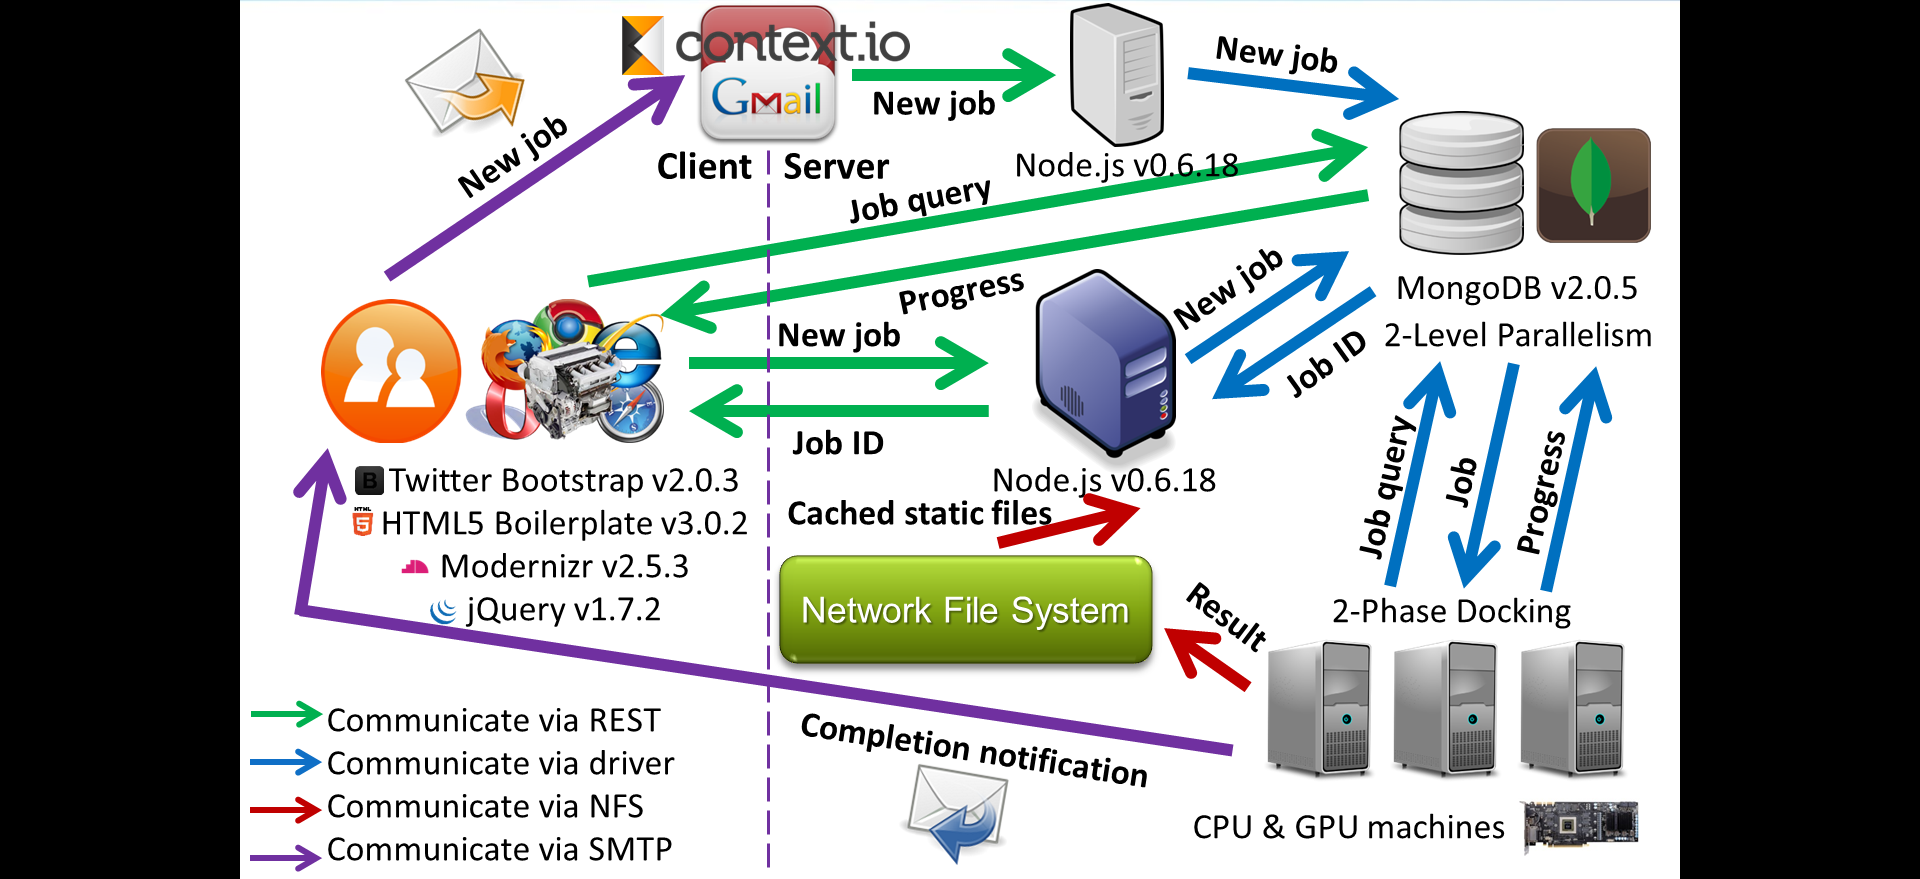
\includegraphics[width=1.0\linewidth]{istar/Architecture.png}
\caption{istar architecture.}
\label{istar:Architecture}
\end{figure}

istar establishing web sites for online virtual screening and drug synthesis, using HTML5 and CSS3 as front end presentation technologies, and node.js and NoSQL databases as back end management implementations.

\begin{figure}
\centering
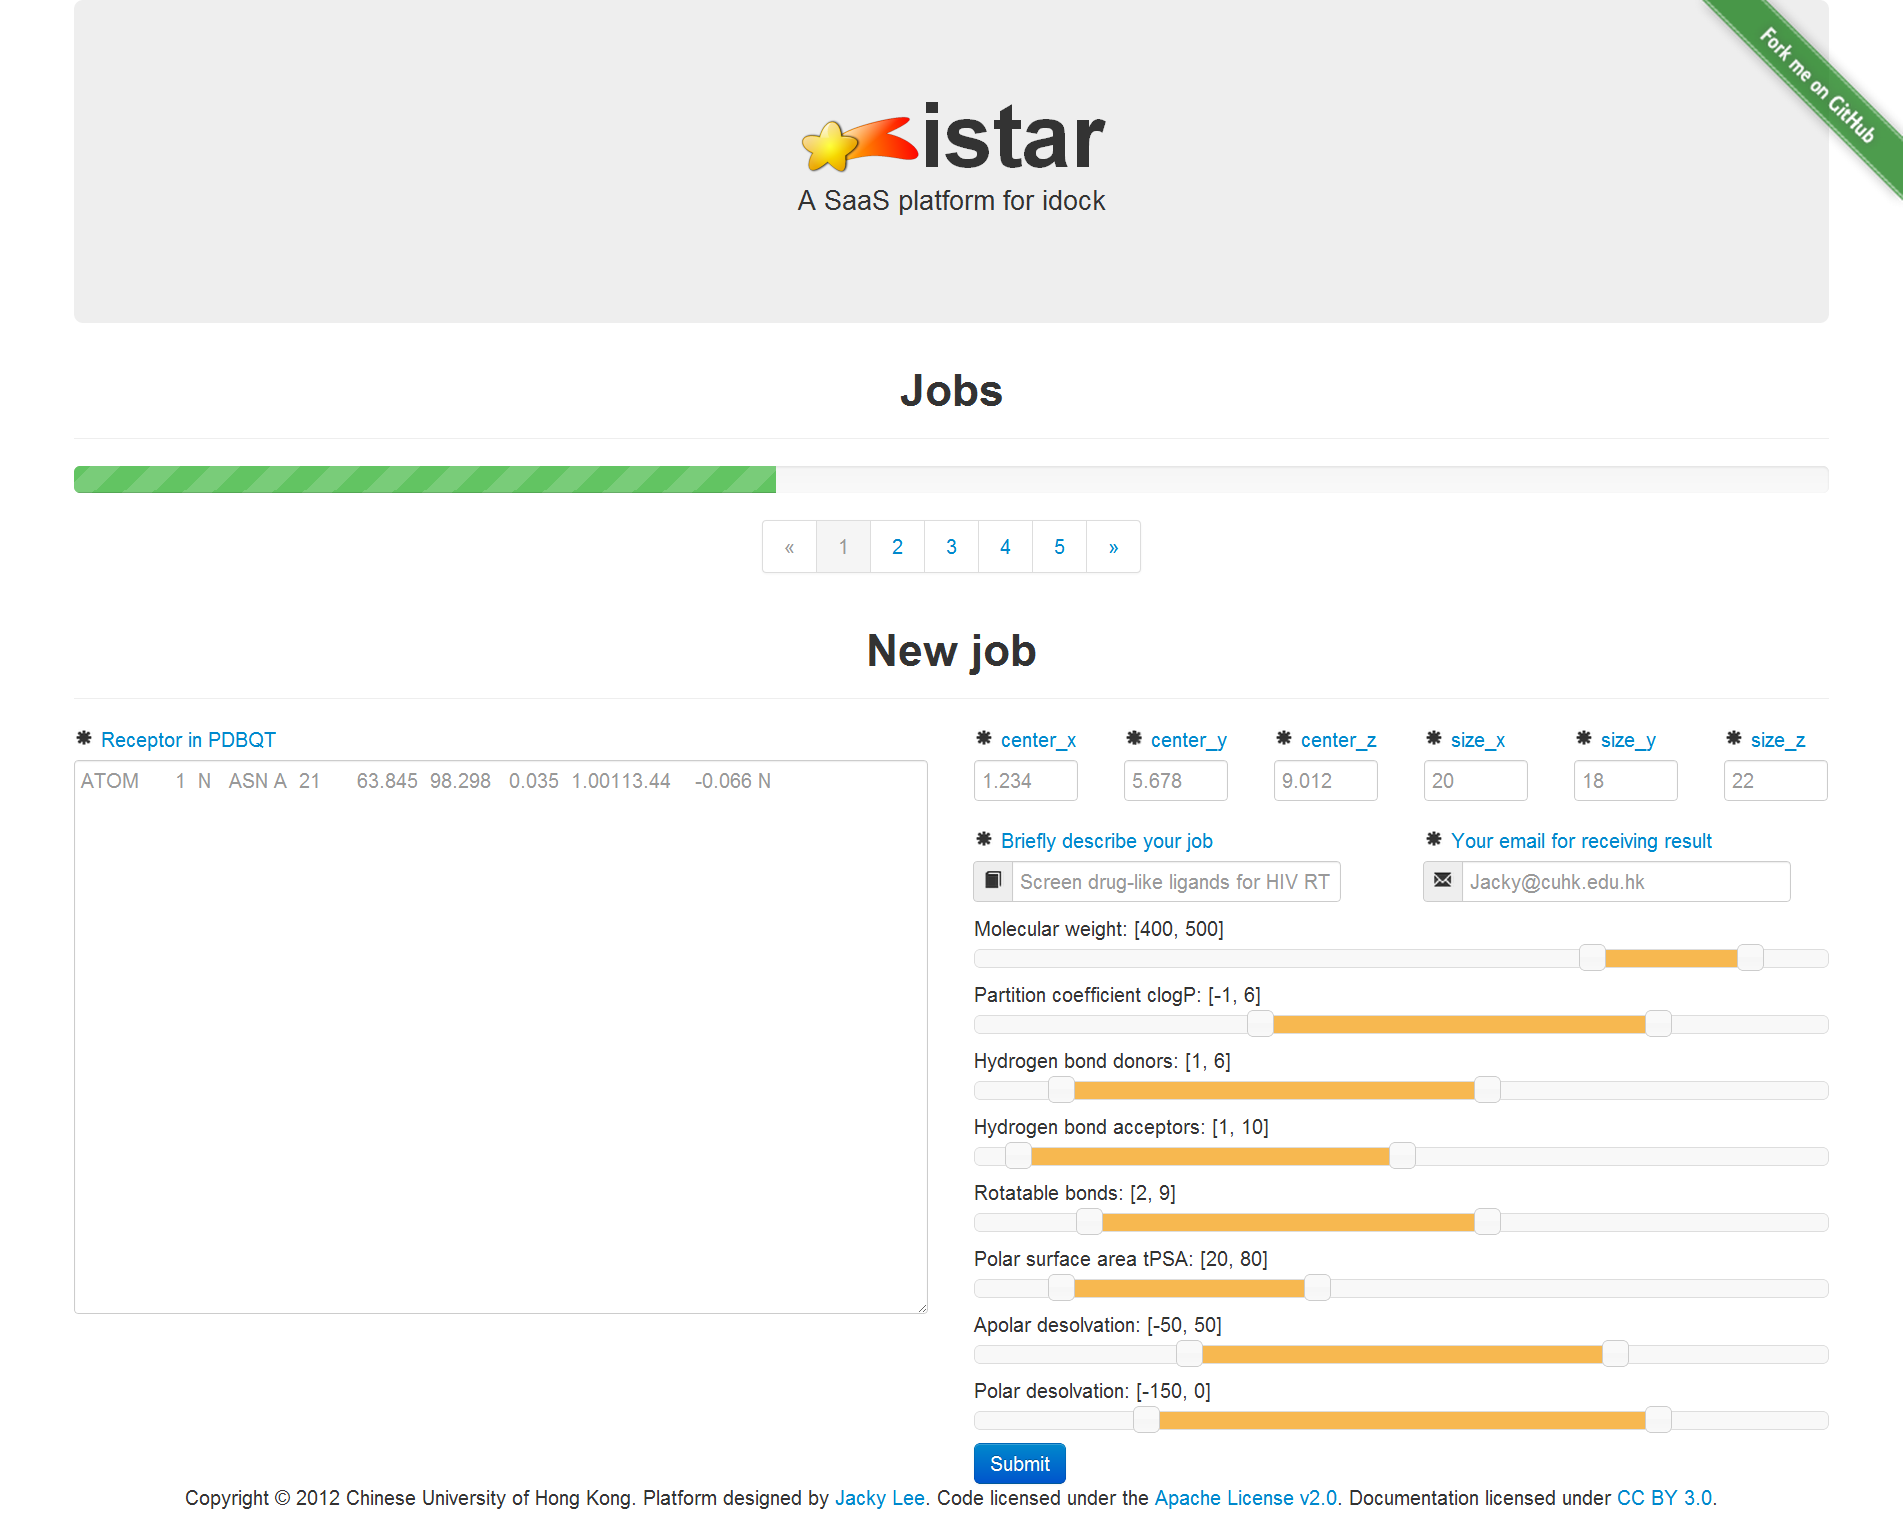
\includegraphics[width=1.0\linewidth]{istar/Website.png}
\caption{istar web site.}
\label{istar:Website}
\end{figure}

\begin{figure}
\centering
\subfloat[Job-level parallelism.]
{
  \label{istar:JobLevelParallelism}
  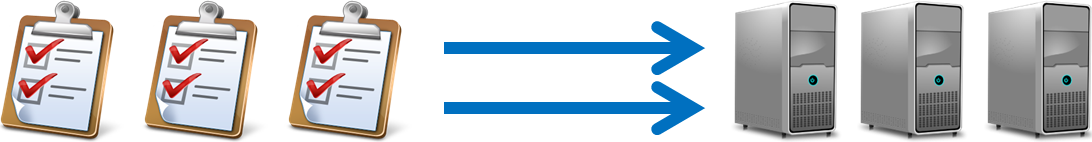
\includegraphics[width=1.0\linewidth]{istar/JobLevelParallelism.png}
}
\\
\subfloat[Slice-level parallelism.]
{
  \label{istar:SliceLevelParallelism}
  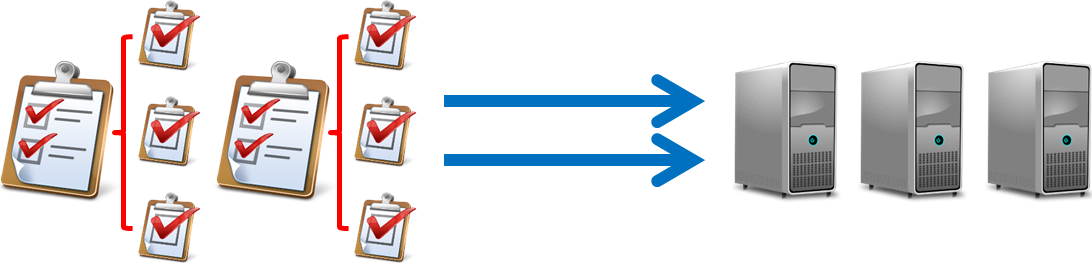
\includegraphics[width=1.0\linewidth]{istar/SliceLevelParallelism.png}
}
\caption{istar 2-level parallelism.}
\label{istar:2LevelParallelism}
\end{figure}

\begin{figure}
\centering
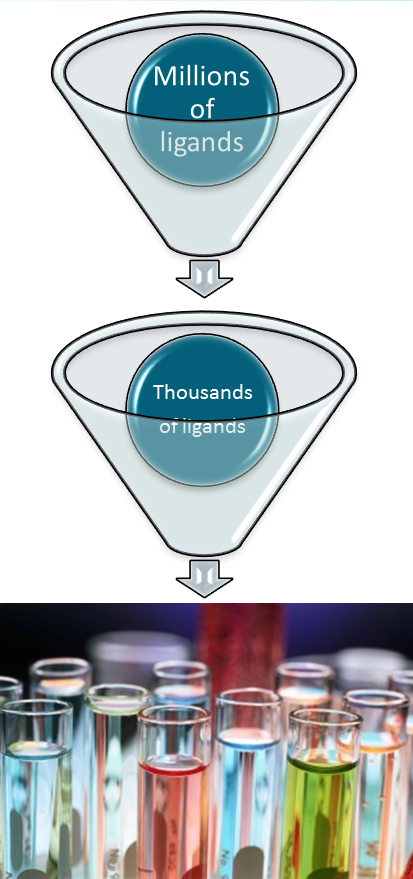
\includegraphics[width=1.0\linewidth]{istar/2PhaseDocking.png}
\caption{istar 2-phase docking.}
\label{istar:2PhaseDocking}
\end{figure}

\section{GPU Acceleration}

For structure-based virtual screening, the most time consuming part is docking. Hence we plan to port idock to GPU, hoping to gain further speedup. This idea is feasible because there are GPU implementations of some other docking programs \citep{723,652,779}, and we also have expertise in GPU programming.

porting idock to CUDA/OpenCL to utilize the huge computational power of NVIDIA/AMD's GPUs.
Kepler GK110
GCN.

\section{Pharmaceutial Applications}

applying idock and igrow for practical drug discovery applications, CCRK, Wnt, Influenza A H1N1

\section{Click Chemistry}

For computational synthesis of potent ligands, even though igrow implements Lipinski's \textit{Rule of Five}, it neglects selectivity, ADMET properties and other drug-like properties, possibly resulting in a high false positive rate. We plan to integrate igrow and ADMET prediction methods into idock to gain speedup and compose a uniform interface.

integrating idock and igrow into one single program to realize grid map caching and partial docking, click chemistry

\section{ADMET Property Prediction}

It was estimated that 40\% to 60\% of new chemical entity (NCE) failures can be attributed to poor ADMET (absorption, distribution, metabolism, excretion, and toxicity) profiles.

PKKB (PharmacoKinetics Knowledge Base) \citep{1133} provides the most extensive collection of freely available data for ADMET properties up to date. PKKB integrates 31,412 experimental or predicted values for 1,685 drug and drug-like molecules from published literature with available experimental ADMET properties including partition coefficient (logP), solubility (logS), intestinal absorption, Caco-2 permeability, human bioavailability, plasma protein binding, volume of distribution, distribution of blood, half-time, excretion, urinary excretion, clearance, toxicity, etc. (Table \ref{PKKB:Properties})

\begin{table}
\centering
\begin{tabular*}
{\linewidth}
{@{\extracolsep{\fill}}rlr}
\toprule
No. & Property & Measurements \\
\midrule
\multicolumn{3}{l}{\textbf{Molecular properties}}\\
1 & Molecular weight & 1,684 \\
2 & logP (experiment) & 1,019 \\
3 & logP (predicted, AB/logP v2.0) & 1,625 \\
4 & Pka & 638 \\
5 & logD (pH=7,predicted) & 1,625 \\
6 & Solubility (experiment) & 800 \\
7 & logS (predicted, ACD/Labs)(pH=7) & 1,614 \\
8 & logSw (predicted, AB/LogSw 2.0) & 1,625 \\
9 & Sw (mg/ml) (predicted, ACD/Labs) & 1,613 \\
10 & Sw (predicted) & 1,625 \\
11 & No. of hbond donors & 1,625 \\
12 & No. of hbond acceptors & 1,625 \\
13 & No. of rotatable bonds & 1,625 \\
14 & TPSA & 1,625 \\
\noalign{\smallskip\smallskip}
\multicolumn{3}{l}{\textbf{Pharmacology}}\\
15 & Status & 1,372 \\
16 & Administration & 501 \\
17 & Pharmacology & 1,543 \\
\noalign{\smallskip\smallskip}
\multicolumn{3}{l}{\textbf{Absorption}}\\
18 & Intestinal absorption & 679 \\
19 & Absorption (description) & 699 \\
20 & Caco-2 & 64 \\
21 & Human bioavailability & 992 \\
\noalign{\smallskip\smallskip}
\multicolumn{3}{l}{\textbf{Distribution}}\\
22 & Plasma protein binding & 1058 \\
23 & Volume of distribution(Vd) & 646 \\
24 & D-blood & 66 \\
\noalign{\smallskip\smallskip}
\multicolumn{3}{l}{\textbf{Metabolism}}\\
25 & Metabolism & 1,111 \\
26 & Half-time & 1,116 \\
\noalign{\smallskip\smallskip}
\multicolumn{3}{l}{\textbf{Excretion}}\\
27 & Excretion & 855 \\
28 & Urinary excretion & 281 \\
29 & Clearance & 410 \\
\noalign{\smallskip\smallskip}
\multicolumn{3}{l}{\textbf{Toxicity}}\\
30 & Toxicity & 873 \\
31 & LD50 (rat) & 219 \\
32 & LD50 (mouse) & 243 \\
\bottomrule
\end{tabular*}
\caption{PKKB property measurements.}
\label{PKKB:Properties}
\end{table}

Figure \ref{PKKB:Schema} shows the PKKB schema. Raw data from literature was first converted into proper formats and then integrated into a central ADMET database. A web site is provided for interactive search of ADMET properties given either structure or descriptive text of compounds of interest.

\begin{figure}
\centering
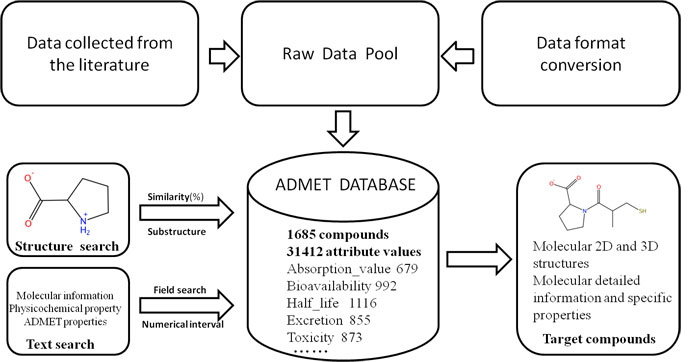
\includegraphics[width=1.0\linewidth]{PKKB/Schema.jpg}
\caption{PKKB schema.}
\label{PKKB:Schema}
\end{figure}

Thanks to the availability of reliable experimental data and basic structural information from PKKB enables, \textit{in silico} ADMET modeling becomes viable. One can predict ADMET properties from chemical structures for a huge number of compounds without actually synthesizing or assaying them.

We propose to make use of advanced machine learning techniques to train a prediction model (Figure \ref{PKKB:Schema}). Once the model is constructed, it is possible to predict ADMET properties of any given compounds. Coupled with conformations and free energy predicted by our tool idock, we can better evaluate a compound from a wide variety of perspectives, leading us to higher drug discovery success rate.

\chapterend
